\section{投机BFT:Ouroboros-BFT与Zyzzyva}
对BFT的高通信复杂度优化的思考引出了一系列所谓投机BFT算法,即,在更强的假设前提下(网络环境更好或拜占庭节点更少)能有更好的性能(performance)。
\subsection{Zyzzyva}
Zyzzyva\cite{kotla2007zyzzyva}由Lorenzo等人在2007年提出,发表在SOSP上并被评为Best Paper。这个命名据说是选取的字典表里的最后一个单词,意味着Zyzzyva是这一系列算法的终结(然而之后还是出现了更好的算法)。

Zyzzyva的协议分为检查点(checkpoint)协议,视图转换(view change)和一致性(agreement)协议。这里我们介绍后两部分。

Zyzzyva其大致结构和定义和PBFT类似,($f$个拜占庭节点,一共$3f+1$个节点,异步网络模型)实现的目标是能有更快的消息复杂度,其核心思想在于在请求的确定被完全确定之前就开始执行。
\subsubsection{流程}
\begin{itemize}
	\item 1. 客户端发送请求给主节点
	\item 2. 主节点接受到请求,给其设置编号,并将请求广播到所有副本节点。
	\item 3. 副本节点接收到有序(ordered)请求,并投机的执行它们,并且给客户点发送回复。
	\item 4. 客户端开始接受副本节点发出的回复,根据\emph{一定时间内}收到的回复数量可以分为下面三种情形:
	   \begin{itemize}
	   	    \item 4a. 若客户端收到$3f+1$个回复(和他的请求匹配的),则认为请求被成功执行,完成请求(complete the request)
	   	    \item 4b. 若客户端收到的回复个数在$2f+1$和$3f$之间,则其生成一个commit信息(包含发送这$2f+1$个回复的节点的ID,签名,请求内容等),并广播给所有的副本节点
	   	        \begin{itemize}
	   	    	\item 4b.1 当副本节点接收到一个合法的commit信息时,生成一个local-commit信息并发送给客户端(若收到的commit信息包含的记录和本地记录不一致,则发起view change(更换主节点))
	   	    	\item 4b.2 当客户端收到$2f+1$个合法的local-commit信息时,完成请求。系统能保证即使存在view change,所有诚实的副本节点都会执行请求。(若客户端在限定时间内没有收到$2f+1$个local-commit信息则跳入4c步骤)
	   	    	\end{itemize}
	   	    \item 4c. 若客户端收到的回复个数少于$2f+1$个,则客户端将请求重新发送给所有副本节点并抄送给主节点(以获得序号)。
	   	     \begin{itemize}
	   	    \item 4c.1 当副本节点收到客户端的请求信息时,若该请求拥有最高的时间戳(timestamp),	则副本节点再发送一个confirm-req信息给主节点$p$并开始计时。若在限定时间内收到主节点发送的有序请求(order-req),则如前所述正常执行该请求。若在限定时间内没有收到,则发起view change,同时将confirm-req广播到所有副本节点。\footnote{注意到这里出现了$n^2$级别消息传输复杂度。}副本节点收到confirm-req时向发送方发送从主节点发来的有序请求。
	   	    \item 4c.2 当主节点收到confirm-req信息时,主节点如第二步所述发送有序请求。
	   	    \end{itemize}
	   	    \item 4d 当客户端发现请求不一致时,发送proof-of-mistake(POM)给所有副本节点并开始view change。(文章提到发起view change并不会影响请求被执行)
	   	\end{itemize}	
\end{itemize}

Zyzzyva的视图转换协议运作当且仅当下面两种情况发生
\begin{itemize}
	\item 当主节点查出有拜占庭行为
	\item 当$f+1$个节点发起view change(文中的方式为发送i-hate-the-primary信息)
\end{itemize}
\reffig{fig:zyzzyva1}演示了Zyzzyva的一致性流程。

\begin{figure}
	\centering
	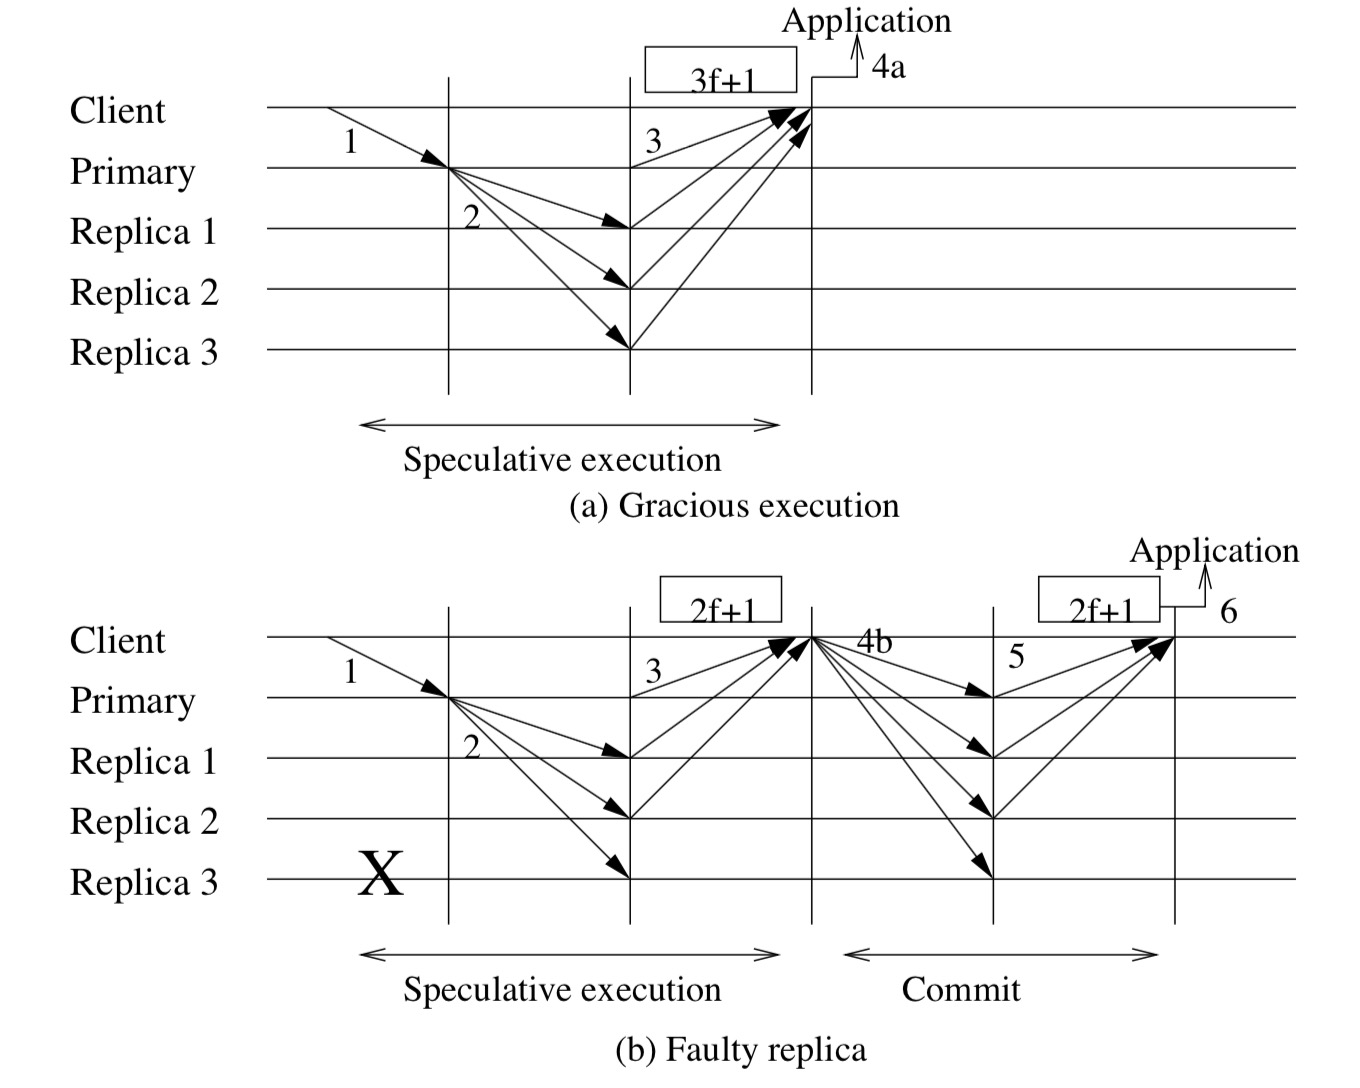
\includegraphics[width=1\textwidth]{../common/zyzzyva_1.png}
	\caption{TPS与安全系数的变化} 
	\label{fig:zyzzyva1}
\end{figure}

文章之后给出了安全性及一致性的证明,以及用实验对比PBFT的性能。这里不详细介绍。

\subsubsection{总结}
Zyzzyva和PBFT相比,运气好的时候执行的更快,但是当主节点更换频繁时效果可能更差。

值得一提的是,Zyzzyva团队之后又提出了致力于在更多的拜占庭故障发生时也能保持高性能的算法,发表在2009年NSDI上,称作Aardvark,据说是字典表的第一个单词(表达他们已经经历了一个轮回)。

